\chapter{Aufbau}

\section{Komponenten}

Das Projekt besteht aus insgesamt \textbf{4 Komponenten}. Nicht alle Komponenten sind für den Endnutzer direkt zugänglich, einige sind auch dem Personal eines Restraurants, welches Sokka verwendet, vorbehalten.

\begin{itemize}
    \item \textbf{Server}: Der Server verwaltet die Daten des Systems und agiert als Kern von Sokka. Alle anderen Komponenten greifen auf den Server zu und stellen Anfragen an diesen.
    \item \textbf{Client}: Der Client ist eine Smartphone-App, welche Kunden des Restaurants installieren können. Durch den Client können verfügbare Produkte eingesehen und bestellt werden.
    \item \textbf{ACP}: Das Admin-Control-Panel ist eine passwortgeschütze Website für das Personal des Restaurants. Über dieses ist es möglich, die Systeminhalte wie Produkte, Menüs und Nutzer zu bearbeiten.
    \item \textbf{Admin-Client}: Der Admin-Client ist eine Smartphone-App, welche vom Personal des Restaurants installiert werden kann. Mit dem Admin-Client können Bestellungen durch Scannen eines QR-Codes von der Client App geprüft und eingelöst werden.
\end{itemize}

Die genaue Funktionsweise der einzelnen Komponenten wird in den folgenden Teilen der Diplomschrift noch genauer beschrieben.

\section{Testumgebung}

Zum Testen der Komponenten wurde ein virtueller Server bei der Hetzner Online GmbH angemietet. Dieser fungierte als Host für den \textit{Server} und dem \textit{ACP}. Der \textit{Client} und der \textit{Admin-Client} benötigen keinen Server, da sie als App direkt auf Smartphones laufen.

\begin{figure}[ht]
    \centering
    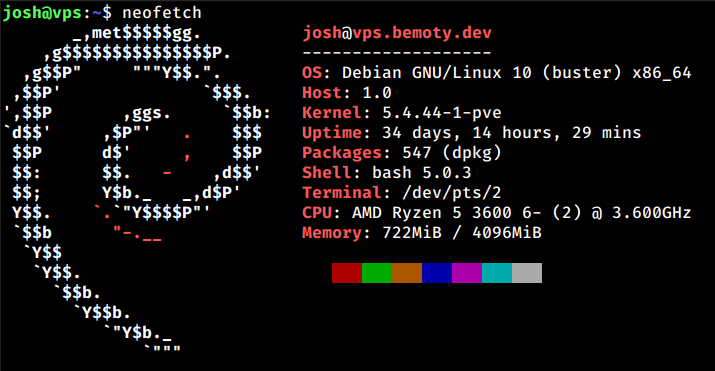
\includegraphics[width=0.55\textwidth]{images/Intro/specs.png}
    \caption{\lstinline{neofetch}: Spezifikationen des Test-VServers}
\end{figure}

Um Zugriff auf die Komponenten zu ermöglichen wurde die Domain \lstinline{sokka.me} beim US-amerikanischen Domain-Registrar Namecheap registriert. Es wurden Nameserver von CloudFlare verwendet, um entsprechende Subdomains für die Komponenten zu hosten. Während der Entwicklung wurden folgende Subdomains verwendet:

\begin{itemize}
    \item \textbf{api.sokka.me}: Über diese Domain erfolgte der Zugriff auf den Server und dessen REST-API.
    \item \textbf{acp.sokka.me}: Das Interface für das ACP konnte über diese Domain erreicht werden.
    \item \textbf{pma.sokka.me}: Eine phpMyAdmin-Instanz konnte über diese Domain erreicht werden. Diese war oftmals zum Debugging der Datenbank sehr hilfreich.
\end{itemize}
